%%%%%%%%%%%%%%%%%%%%%%%%%%%%%%%%%%%%%%%%%%%%%%%%%%%%%%%%%%%%%%%%%%%%%%%%%%%%%
%% Original default rstudio/pandoc latex file
%% upated by @jhollist 09/15/2014
%% inspired by @cboetting https://github.com/cboettig/template and
%% @rmflight blog posts:
%% http://rmflight.github.io/posts/2014/07/analyses_as_packages.html 
%% http://rmflight.github.io/posts/2014/07/vignetteAnalysis.html).  
%%%%%%%%%%%%%%%%%%%%%%%%%%%%%%%%%%%%%%%%%%%%%%%%%%%%%%%%%%%%%%%%%%%%%%%%%%%%%

\documentclass[11pt,a4paper]{article}
\usepackage[T1]{fontenc}
\usepackage{lmodern}
\usepackage{amssymb,amsmath}
\usepackage{ifxetex,ifluatex}
\usepackage{fixltx2e} % provides \textsubscript
% use upquote if available, for straight quotes in verbatim environments
\IfFileExists{upquote.sty}{\usepackage{upquote}}{}
\ifnum 0\ifxetex 1\fi\ifluatex 1\fi=0 % if pdftex
  \usepackage[utf8]{inputenc}
\else % if luatex or xelatex
  \ifxetex
    \usepackage{mathspec}
    \usepackage{xltxtra,xunicode}
  \else
    \usepackage{fontspec}
  \fi
  \defaultfontfeatures{Mapping=tex-text,Scale=MatchLowercase}
  \newcommand{\euro}{€}
\fi
% use microtype if available
\IfFileExists{microtype.sty}{\usepackage{microtype}}{}
\usepackage[margin=1in]{geometry}
\usepackage{longtable,booktabs}
\usepackage{graphicx}
% Redefine \includegraphics so that, unless explicit options are
% given, the image width will not exceed the width of the page.
% Images get their normal width if they fit onto the page, but
% are scaled down if they would overflow the margins.
\makeatletter
\def\ScaleIfNeeded{%
  \ifdim\Gin@nat@width>\linewidth
    \linewidth
  \else
    \Gin@nat@width
  \fi
}
\makeatother
\let\Oldincludegraphics\includegraphics
{%
 \catcode`\@=11\relax%
 \gdef\includegraphics{\@ifnextchar[{\Oldincludegraphics}{\Oldincludegraphics[width=\ScaleIfNeeded]}}%
}%
\ifxetex
  \usepackage[setpagesize=false, % page size defined by xetex
              unicode=false, % unicode breaks when used with xetex
              xetex]{hyperref}
\else
  \usepackage[unicode=true]{hyperref}
\fi
\hypersetup{breaklinks=true,
            bookmarks=true,
            pdfauthor={},
            pdftitle={Agreement Attraction in Turkish: Effects of Nominal and Verbal Plural Morphemes},
            colorlinks=true,
            citecolor=blue,
            urlcolor=blue,
            linkcolor=magenta,
            pdfborder={0 0 0}}
\urlstyle{same}  % don't use monospace font for urls
\setlength{\parindent}{0pt}
\setlength{\parskip}{6pt plus 2pt minus 1pt}
\setlength{\emergencystretch}{3em}  % prevent overfull lines
\setcounter{secnumdepth}{5}

%%%%%%%%%%%%%%%%%%%%%%%%%%%%%%%%%%%%%%%%%%%%%%%%%%%%%%%%
%Changes borrowed from @cboettig, added by @jhollist 
% A modified page layout 
\textwidth 6.75in
\oddsidemargin -0.15in
\evensidemargin -0.15in
\textheight 9in
\topmargin -0.5in
\usepackage{lineno} % add 
  \linenumbers % turns line numbering on 
%%%%%%%%%%%%%%%%%%%%%%%%%%%%%%%%%%%%%%%%%%%%%%%%%%%%%%%%

%%%%%%%%%%%%%%%%%%%%%%%%%%%%%%%%%%%%%%%%%%%%%%%%%%%%%%%%
%%Packages and layout changes by @jhollist 09/15/2014
\usepackage{ragged2e}
\usepackage[font=normalsize]{caption}
  \usepackage[singlespacing]{setspace}
\usepackage{parskip}
\usepackage{fancyhdr}
\pagestyle{fancy}
\fancyhf{}
\renewcommand{\headrulewidth}{0pt}
  \rfoot{\today}
\lfoot{\thepage}
%%Changed default abstract width and added lines
\renewenvironment{abstract}{
  \hfill\begin{minipage}{1\textwidth}
  \rule{\textwidth}{1pt}\vspace{5pt}
  \normalsize
  \begin{justify}
  \bfseries\abstractname\vspace{5pt}
  \end{justify}}
  {\par\noindent\rule{\textwidth}{1pt}\end{minipage}
}
%%%%%%%%%%%%%%%%%%%%%%%%%%%%%%%%%%%%%%%%%%%%%%%%%%%%%%%%

\title{Agreement Attraction in Turkish: Effects of Nominal and Verbal Plural
Morphemes}
\author{
Utku Turk
Pavel Logacev
}
\date{}
% Allowing for landscape pages
\usepackage{lscape}
\newcommand{\blandscape}{\begin{landscape}}
\newcommand{\elandscape}{\end{landscape}}

% Left justification of the text: see https://www.sharelatex.com/learn/Text_alignment
% \usepackage[document]{ragged2e} % already in the latex template
\newcommand{\bleft}{\begin{flushleft}}
\newcommand{\eleft}{\end{flushleft}}

% multicols
\usepackage{multicol}
\usepackage{paracol}

% enumerated examples
\usepackage{enumitem}

% for linguistic examples &  interlinear glosses
\usepackage{gb4e}
\exewidth{(10.159)}
\noautomath
\let\eachwordone=\it

\usepackage{qtree}

%%Fix tightlist error: https://stackoverflow.com/questions/40438037/tightlist-error-using-pandoc-with-markdown
%%Added 2018-03-26 
\providecommand{\tightlist}{%
  \setlength{\itemsep}{0pt}\setlength{\parskip}{0pt}}
%%%  
  

\begin{document}
%%Edited by @jhollist 09/15/2014
%%Adds title from YAML
\begin{singlespace}
\begin{center}
\huge Agreement Attraction in Turkish: Effects of Nominal and Verbal Plural
Morphemes
\end{center}
%%Adds Author, correspond email asterisk, and affilnum from YAML
\begin{center}
\large
Utku Turk \textsuperscript{*} \textsuperscript{1} 
Pavel Logacev \textsuperscript{1} 
\end{center}
%%Adds affiliations from YAML
\begin{justify}
\footnotesize \emph{ 
\\*
\textsuperscript{1}Bogazici University, South Campus, John Freely Building, Department of
Linguistics, 34342, Istanbul, Turkey\\*
}
%%Adds corresponding author email(s) from YAML
\newcounter{num}
\setcounter{num}{1}
\\[0.1cm]
\footnotesize \emph{ 
\ifnum\value{num}=1%
\textsuperscript{*} corresponding author:
\fi
\href{mailto:utku.turk@boun.edu.tr}{\nolinkurl{utku.turk@boun.edu.tr}}
\stepcounter{num}
}
\end{justify}
%%Adds date from YAML
\normalsize

\end{singlespace}


\vspace{2mm}\hrule

In this paper, our objective is to explore the source of agreement
attraction effects in Turkish found by Lago (2018). The interpretation
of their finding is complicated by the fact that in their possessive
form all head nouns in their stimuli are morphologically ambiguous
between possessive and accusative. Due to the mismatch in the frequency
of usage of accusative and genitive, which is used as a attractor in
this experiment, as a controller, Lago (2018)'s findings could
potentially be explained with occasional shallow processing. We have
replicated Lago (2018)'s experiment with unambigious head nouns, and we
have found the same agreement attraction effects. However, this may mean
that participants may engage in even more shallow processing than we
imagined. We postulate that participants solely check for the presence
of a \emph{-lAr} morpheme, while largely disregarding the remainder of
the sentence. We utilize an experiment design in which we use a relative
clause with or without plural agreement on the verb in place of the
genitive possessor since both verbal and nominal plural morphemes are
the same in Turkish. If participants did, in fact, adopt a superficial
processing strategy, we would expect to find a number agreement
attraction effect similar in magnitude to Lago (2018)'s. However, if
number attraction is not an artifact of shallow processing strategies,
we should expect to find no number attraction in this experiment.

\vspace{3mm}\hrule

\emph{Keywords}: Turkish, agreement attraction, task effect, shallow
processing

\bleft

\hypertarget{introduction}{%
\section{INTRODUCTION}\label{introduction}}

Attraction errors in production and comprehension of subject-verb
agrrement, in which a verb does not agree with the grammatical agreement
controller, but with a potential attractors, have been the focal point
of many research for quite a long time. In fact, it is still a widely
researched are in psycholinguistic studies. Despite the thorough
research that has been carried out, studies that have been conducted on
agreement attraction in Turkish have been extremely few. In fact, Lago
(2018) has been the only study to look into this phenomenon in Turkish.
Lago (2018)'s study make use of genitive-possessive structures in the
subject position, in which the possessive-marked noun is the head of the
noun phrase which acts as the grammatical agreement controller, and the
genitive noun serves as a potential attractor. In a speeded
acceptability judgment study, they found a significant effect of number
agreement attraction. However, the interpretation of their finding may
be a result of a non-subjecthood cues originating from their use of
morphologically ambiguous forms of possessive. In their possessive form
all head nouns in their stimuli are ambigiuous between possessive and
accusative.

In Turkish, accusative number agreement controllers are extremely rare,
while genitive agreement controllers are very frequent. Thus, Lago
(2018)'s finding could possibly be explained by occasional shallow
processing. When all syntactic relations in the sentence were processed
fully, the possessive noun should have been identified as the
controller. Meanwhile the genitive noun may sometimes have been
erroneously identified as the controller during shallow processing,
because genitives are more likely to act as agreement controllers than
accusatives. A second alternative explanation of Lago (2018)'s finding
may be the fact that participants may engage in even more shallow
processing than outlined above. Participants may have erroneously
responded \emph{Yes} on some trials due to (i) the presence of a plural
morpheme on a noun (attractor or controller) and (ii) the presence of a
plural agreement morpheme on the verb. We speculate that on such trials,
participants would have simply tried to check for the presence of such
morphemes, while largely disregarding the remainder of the sentence.

We first replicated Lago (2018)'s experiment with unambiuous head nouns.
To this end, we have revised the items that were used previously, to
avoid morphological ambiguity between possessive and accusative forms.
The effect found by Lago (2018) replicates with unambiguous nouns as
discused in \S 2.

\S 3 discussses the alternative account that posits even more shallow
processing as mentioned above and offers a pre-registered experiment
using RC attractors with possible outcomes and their indications. Since
both nominal and verbal plural morphemes in Turkish take on the same
form (\emph{-ler} or \emph{-lar} depending on the phonological
environment), we can test this possibility with an experiment, in which
we use relative clause with or without plural agreement on the verb in
the place of the genitive possessors. An agreement attraction effect
similar in magnitude to Lago (2018)'s would mean that participants use
aforementioned strategies.

\S 4 presents a discussion revolving around possible Lastly, \S 5 offers
a brief conclusion and presents topics for future researches.

\hypertarget{replicaton-of-lago}{%
\section{REPLICATON OF Lago (2018)}\label{replicaton-of-lago}}

In their study, Lago (2018) investigated the comprehension of
subject-verb agreement in Turkish-German bilinguals and Turkish
monolinguals. They used speeded acceptability judments for the effects
of number attraction in Turkish. Their sentences makes us of
genitive-possessive constructions in the subject position, where the
genitive is the attractor and the possessive is the head noun. They have
manipulated the grammaticality of the sentence by changing the plural
morphology of the verb, and they also manipulated the plurality of the
attractor noun. In grammatical conditions, subject and the verb both
bears the singular morphology with no overt morpheme. Moreover, in the
ungrammatical conditions the verb bears the overt \emph{-lAr} morpheme
whereas the subject is still singular as exemplified below.

\begin{exe}
\ex
\begin{xlist}
\ex \underline{Grammatical, SG attractor} \label{lago1}
\gll \c{S}ark{\i}c{\i}-n{\i}n vokalist-i sahne-de s\"{u}rekli z{\i}pla-d{\i}\\
singer-\textsc{gen} vocalist-\textsc{poss} stage-\textsc{loc} non-stop jump-\textsc{pst}-$\varnothing$\\
\glt The singer's backup vocalist jumped on the stage non-stop.

\ex \underline{Grammatical, PL attractor} \label{lago2}
\gll \c{S}ark{\i}c{\i}-lar-{\i}n vokalist-i sahne-de s\"{u}rekli z{\i}pla-d{\i}\\
singer-\textsc{pl}-\textsc{gen} vocalist-\textsc{poss} stage-\textsc{loc} non-stop jump-\textsc{pst}-$\varnothing$\\
\glt The singer's backup vocalist jumped on the stage non-stop.

\ex \underline{Ungrammatical, PL attractor} \label{lago3}
\gll \c{S}ark{\i}c{\i}-lar-{\i}n vokalist-i sahne-de s\"{u}rekli z{\i}pla-d{\i}-lar.\\
singer-\textsc{pl}-\textsc{gen} vocalist-\textsc{poss} stage-\textsc{loc} non-stop jump-\textsc{pst}-\textsc{3Pl}\\
\glt The singer's backup vocalist jumped on the stage non-stop.

\ex \underline{Ungrammatical, SG attractor} \label{lago4}
\gll \c{S}ark{\i}c{\i}-n{\i}n vokalist-i sahne-de s\"{u}rekli z{\i}pla-d{\i}-lar.\\
singer-\textsc{gen} vocalist-\textsc{poss} stage-\textsc{loc} non-stop jump-\textsc{pst}-\textsc{3Pl}\\
\glt The singer's backup vocalist jumped on the stage non-stop.
\end{xlist}
\end{exe}

They have found a significant effect of number attraction in Turkish
ranging between 11\%--15\% across monolinguals. As seen from the results
of statistical analysis in Table (\ref{lagomodel}), acceptability
judgments showed an immense effect of grammaticality, and there is also
interaction between grammaticality and attractor number which indicates
an number attraction effect.

\begin{table}[]
\centering
\begin{tabular}{llcccc}
\hline
    &                                        & \multicolumn{4}{l}{Monolingual Speakers}                                               \\ \cline{3-6} 
    &                                        & $\beta$        & SE            & \emph{z} & \emph{p} \\ \hline
\multicolumn{2}{l}{\textbf{Attraction Task}} &                &               &                           &                           \\
    & Grammaticality                         & \textbf{-5.51} & \textbf{0.33} & \textbf{-16.69}           & \textbf{.000}             \\
    & Attractor Number                       & 0.14           & 0.25          & 0.57                      & .571                      \\
    & Grammaticality x Attractor Number      & \textbf{1.69}  & \textbf{0.53} & \textbf{3.19}             & \textbf{.001}             \\
    & Attractor Number: Ungram conditions    & \textbf{0.94}  & \textbf{0.26} & \textbf{3.68}             & \textbf{.000}             \\
    & Attractor Number: Gram conditions      & -0.79          & 0.52          & -1.51                     & .131                      \\ \hline
\end{tabular}
\caption{Model results for the judgments of monolingual cited from @Lago.}
\label{lagomodel}
\end{table}

According to Lago (2018)'s stipulation, Turkish genitive case does not
provide a strong cue against subjecthood since it is extremely common to
see genitive marked subjects in Turkish embedded clauses, as in example
(\ref{gensubj}).

\begin{exe}
\ex \label{gensubj}
\gll k\"{o}y-\"{u} bir haydut-un bas-t{\i}\u{g}-{\i}n-{\i} duy-du-m.\\
village-\textsc{acc} a bandit-\textsc{gen} raid-\textsc{nmlz}-\textsc{3Sg}-\textsc{acc} hear-\textsc{pst}-\textsc{1Sg}\\
\glt I heard that a (certain) robber raided the village. (Adapted from Woolford (2009))
\end{exe}

\hypertarget{motivation}{%
\subsection{Motivation}\label{motivation}}

\hypertarget{modifications}{%
\subsection{Modifications}\label{modifications}}

\hypertarget{participants}{%
\subsection{Participants}\label{participants}}

\hypertarget{filler-items}{%
\subsection{Filler Items}\label{filler-items}}

\hypertarget{results-and-discussion}{%
\subsection{Results and Discussion}\label{results-and-discussion}}

\hypertarget{experiment-2-rc-attractor}{%
\section{EXPERIMENT 2: RC ATTRACTOR}\label{experiment-2-rc-attractor}}

\hypertarget{motivation-1}{%
\subsection{Motivation}\label{motivation-1}}

\hypertarget{items-and-fillers}{%
\subsection{Items and Fillers}\label{items-and-fillers}}

\hypertarget{expectations}{%
\subsection{Expectations}\label{expectations}}

\hypertarget{possible-outcomes-and-discussion}{%
\subsection{Possible Outcomes and
Discussion}\label{possible-outcomes-and-discussion}}

\hypertarget{discussion}{%
\section{DISCUSSION}\label{discussion}}

Discuss.

\hypertarget{conclusions}{%
\section{CONCLUSIONS}\label{conclusions}}

Intro and repeat.

\hypertarget{acknowledgements}{%
\section{ACKNOWLEDGEMENTS}\label{acknowledgements}}

We used the statistical language \texttt{R} (R Core Team 2018) for all
our analyses. These were implemented in dynamic rmarkdown documents
using \texttt{knitr} (Xie 2014, 2015, 2018) and \texttt{rmarkdown}
(Allaire et al. 2018, Xie et al. 2018) packages. All graphs have been
done with \texttt{ggplot} (Wickham 2016). Thank the Mine and Kadir for
their student from courses.

\hypertarget{references}{%
\section{REFERENCES}\label{references}}

\hypertarget{refs}{}
\leavevmode\hypertarget{ref-Allaire_2018}{}%
Allaire, J., Y. Xie, J. McPherson, J. Luraschi, K. Ushey, A. Atkins, H.
Wickham, J. Cheng, W. Chang, and R. Iannone. 2018. Rmarkdown: Dynamic
documents for r.

\leavevmode\hypertarget{ref-Lago}{}%
Lago, S. 2018. Straight from the horse's mouth: agreement attraction
effects with Turkish possessors.

\leavevmode\hypertarget{ref-R_Core_Team_2018}{}%
R Core Team. 2018. R: A language and environment for statistical
computing. R Foundation for Statistical Computing, Vienna, Austria.

\leavevmode\hypertarget{ref-Wickham_2016}{}%
Wickham, H. 2016. Ggplot2: Elegant graphics for data analysis.
Springer-Verlag New York.

\leavevmode\hypertarget{ref-woolford}{}%
Woolford, E. 2009. Differential subject marking at argument structure,
syntax, and pf. Pages 17--40 \emph{in} Differential subject marking.
Springer.

\leavevmode\hypertarget{ref-Xie_2014}{}%
Xie, Y. 2014. Knitr: A comprehensive tool for reproducible research in
R. \emph{in} V. Stodden, F. Leisch, and R. D. Peng, editors.
Implementing reproducible computational research. Chapman; Hall/CRC.

\leavevmode\hypertarget{ref-Xie_2015}{}%
Xie, Y. 2015. Dynamic documents with R and knitr. 2nd editions. Chapman;
Hall/CRC, Boca Raton, Florida.

\leavevmode\hypertarget{ref-Xie_2018}{}%
Xie, Y. 2018. Knitr: A general-purpose package for dynamic report
generation in r.

\leavevmode\hypertarget{ref-Xie_2018a}{}%
Xie, Y., J. Allaire, and G. Grolemund. 2018. R markdown: The definitive
guide. Chapman; Hall/CRC, Boca Raton, Florida.

\eleft

\clearpage

\listoftables

\newpage

\begin{longtable}[]{@{}rrrrl@{}}
\caption{A glimpse of the famous \emph{Iris} dataset.}\tabularnewline
\toprule
Sepal.Length & Sepal.Width & Petal.Length & Petal.Width &
Species\tabularnewline
\midrule
\endfirsthead
\toprule
Sepal.Length & Sepal.Width & Petal.Length & Petal.Width &
Species\tabularnewline
\midrule
\endhead
5.1 & 3.5 & 1.4 & 0.2 & setosa\tabularnewline
4.9 & 3.0 & 1.4 & 0.2 & setosa\tabularnewline
4.7 & 3.2 & 1.3 & 0.2 & setosa\tabularnewline
4.6 & 3.1 & 1.5 & 0.2 & setosa\tabularnewline
5.0 & 3.6 & 1.4 & 0.2 & setosa\tabularnewline
5.4 & 3.9 & 1.7 & 0.4 & setosa\tabularnewline
\bottomrule
\end{longtable}

\newpage

\begin{longtable}[]{@{}lrrrrrrrrrrr@{}}
\caption{Now a subset of mtcars dataset.}\tabularnewline
\toprule
& mpg & cyl & disp & hp & drat & wt & qsec & vs & am & gear &
carb\tabularnewline
\midrule
\endfirsthead
\toprule
& mpg & cyl & disp & hp & drat & wt & qsec & vs & am & gear &
carb\tabularnewline
\midrule
\endhead
Merc 280 & 19.2 & 6 & 167.6 & 123 & 3.92 & 3.440 & 18.30 & 1 & 0 & 4 &
4\tabularnewline
Merc 280C & 17.8 & 6 & 167.6 & 123 & 3.92 & 3.440 & 18.90 & 1 & 0 & 4 &
4\tabularnewline
Merc 450SE & 16.4 & 8 & 275.8 & 180 & 3.07 & 4.070 & 17.40 & 0 & 0 & 3 &
3\tabularnewline
Merc 450SL & 17.3 & 8 & 275.8 & 180 & 3.07 & 3.730 & 17.60 & 0 & 0 & 3 &
3\tabularnewline
Merc 450SLC & 15.2 & 8 & 275.8 & 180 & 3.07 & 3.780 & 18.00 & 0 & 0 & 3
& 3\tabularnewline
Cadillac Fleetwood & 10.4 & 8 & 472.0 & 205 & 2.93 & 5.250 & 17.98 & 0 &
0 & 3 & 4\tabularnewline
Lincoln Continental & 10.4 & 8 & 460.0 & 215 & 3.00 & 5.424 & 17.82 & 0
& 0 & 3 & 4\tabularnewline
\bottomrule
\end{longtable}

\clearpage

\listoffigures

\newpage

\begin{figure}
\centering
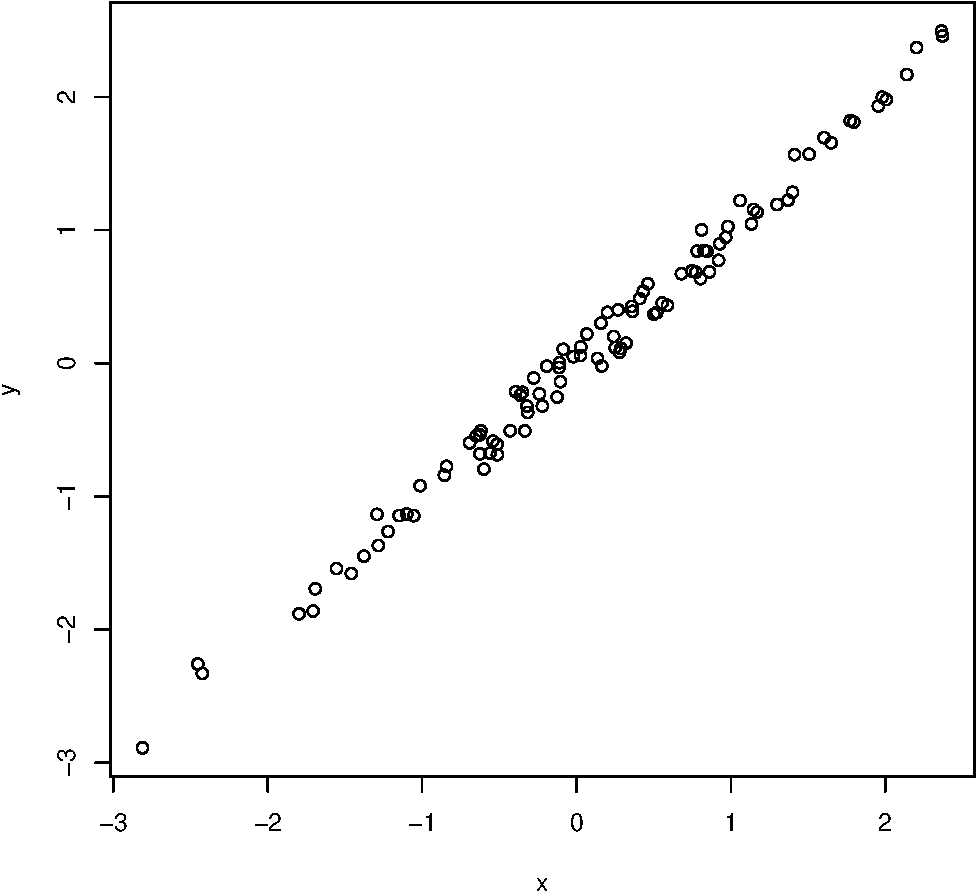
\includegraphics{output/figures/Fig1-1.pdf}
\caption{Just my first figure with a very fantastic caption.}
\end{figure}

\newpage

\blandscape

\begin{figure}
\centering
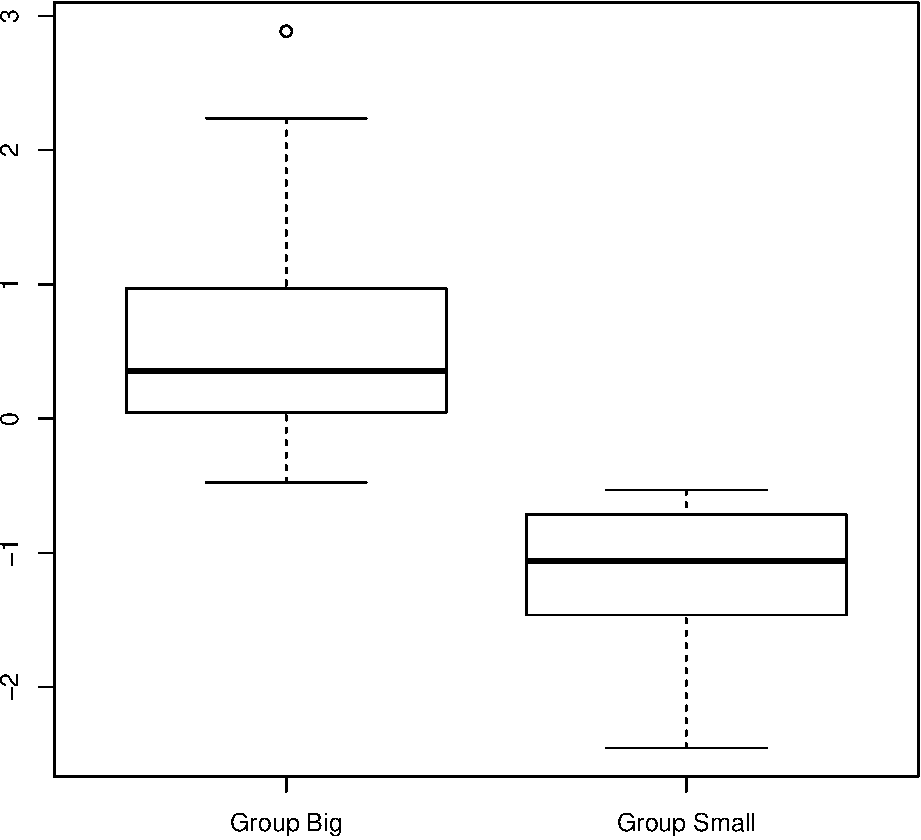
\includegraphics{output/figures/Fig2-1.pdf}
\caption{Second figure in landscape format.}
\end{figure}

\elandscape

\clearpage

\end{document}